\section{Auswertung}

\subsection{Berechnung der Verdampfungswärme im niedrigen Druckbereich}

Mit der Apparatur \ref{fig:figskizze1} wurde im Versuch der Dampfdruck $p$ in $\si{\milli\bar}$ und die Temperatur $T$ in $\si{\celsius}$ gemessen. Die hergeleitete Lösung 
der Clausius-Clapeyron Differentialgleichung \eqref{eqn:wichtig} gibt Aufschluss auf die Verdampfungswärme $L$. Durch eine reziproke Darstellung der Temperaturen und eine Logarithmierung von beiden Seiten
ergibt sich folgender linearer Zusammenhang.

\begin{equation}
\label{eqn:1}
\text{ln}(p) = - \frac{L}{R} \cdot \frac{1}{T} + \text{ln}(p_{0})
\end{equation}
\\
In dieser Geradengleichung ist die Verdampfungswärme $L$ die Steigung und sie kann deshalb durch eine lineare Ausgleichsrechnung gewonnen werden.
Das p-T-Diagramm ist zunächst in Abbildung \ref{fig:plot1} geplottet, dabei wurden die Temperaturen in Kelvin umgerechnet.
\begin{figure}[h]
    \centering
    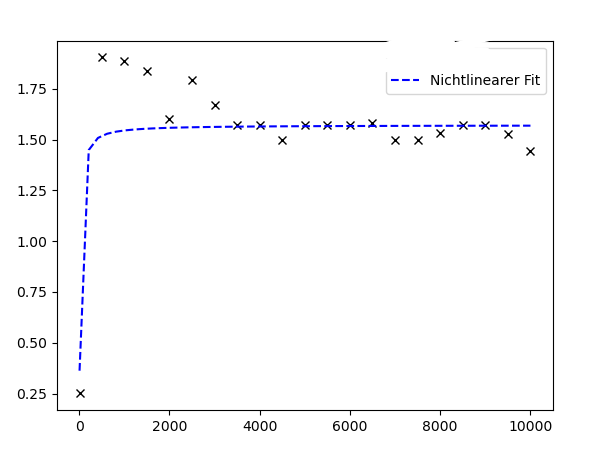
\includegraphics[width=\textwidth]{build/plot1.pdf}
    \caption{Gemessene Dampfdruckkurve bei niedrigen Drücken.}
    \label{fig:plot1}
  \end{figure}
Anschließend können durch Anpassung der Darstellung die Punkte in eine Geradengleichung überführt werden, wie in Gleichung \eqref{eqn:1} gezeigt. 
\\
Anhand einer lineare Regression, beispielsweise mit Python, kann eine Ausgleichsgerade durch die Punkte geplottet werden. Diese ist zusammen mit den Messpunkten in Abbildung \ref{fig:plot2} dargestellt.
\begin{figure}[h]
    \centering
    \includegraphics[width=\textwidth]{build/plot2.pdf}
    \caption{Linearer Fit durch die Messpunkte bei niedrigem Druck.}
    \label{fig:plot2}
\end{figure}
Die Ausgleichsgerade ist von der Form

\begin{equation}
\text{ln}(p) = a \cdot \left( \frac{1}{T}\right) +b
\end{equation}
\\
und die folgenden Parameter ergeben sich.
\begin{align}
a &= \SI{-4710.774(43656)}{\kelvin} \\
b &= \SI{19.492(0133)}{}
\end{align}
Aus dem bereits zuvor genannten Zusammenhang \eqref{eqn:1} folgt nun sofort.

\begin{equation}
a = -\frac{L}{R} \quad \to \quad L = -R \cdot a
\end{equation}
\\
Die universelle Gaskonstante $R$ ist eine exakte Größe und lässt sich der Literatur \cite{Naturkonstanten} entnehmen.
Für die Verdampfungswärme $L$ ergibt sich letztendlich.
\begin{equation}
L = \SI{39.168(0363)}{\kilo\joule\per\mol\per\kelvin}
\end{equation}
Der Fehler auf die Verdampfungswärme entspringt aus der folgenden Gaußschen Fehlerfortpflanzung. Diese ist hier besonders simpel auf Grund des linearen Zusammenhangs zwischen $a$ und $L$. 
\begin{equation}
\increment L = -R \cdot \increment a
\end{equation}

\subsection{Berechnung der Verdampfungswärme im hohen Druckbereich}

Analog zu der vorherigen Auswertung kann hier die Verdampfungswärme $L$ für die ermittelte Dampfdruckkurve im zweiten Teil des Versuchs \ref{fig:figskizze2} errechnet werden.
Die Dampfdruckkurve ist zunächst in Abbildung \ref{fig:plot3} dargestellt.
\begin{figure}[h]
    \centering
    \includegraphics[width=\textwidth]{build/plot3.pdf}
    \caption{Gemessene Dampfdruckkurve bei höheren Drücken.}
    \label{fig:plot3}
\end{figure}
Wie zuvor wird die Darstellung durch Logarithmierung angepasst und eine Ausgleichsgerade ermittelt. Das Ergebnis ist im Diagramm ----
\begin{figure}[h]
    \centering
    \includegraphics[width=\textwidth]{build/plot4.pdf}
    \caption{Linearer Fit durch die Messpunkte bei hohem Druck.}
    \label{fig:plot4}
\end{figure}